\scanpage{63}
\figure{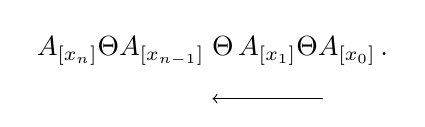
\begin{tikzpicture}
\node at (2,0.6) {$A_{[x_n]}\Theta A_{[x_{n-1}]}\;\unsure{\Theta}\, A_{[x_1]}\Theta A_{[x_0]}\,.$};
\draw[->] (3.4,0)--(2,0);
\end{tikzpicture}}
\figure{\begin{tikzpicture}
\draw (0,1.6)--(2,1.6);\foreach \x in {0,.4,1.6,2} \draw (\x,1.5)--(\x,1.7);
\draw[->,line width=1.2pt] (0,.8)--(1,.8);\draw[dashed] (1,.8)--(1.7,.8);\draw (0,.7)--(0,.9);\draw (1.7,.7)--(1.7,.9);
\draw (0,0)--(1.1,0);\draw[->,thick] (-.6,0)--(0,0);\draw (-.7,-.1)--(-.7,.1);\draw (0,-.1)--(0,.1);\draw (1.1,-.1)--(1.1,.1);
\end{tikzpicture}}
\figure{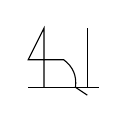
\begin{tikzpicture}[scale=.5]
\draw (0,0)--(1.8,0);\draw (.4,0)--(.4,1.5)--(0,.7)--(.9,.7) to[bend left] (1.2,0)--(1.5,-.2);\draw (1.5,0)--(1.5,1.5);
\end{tikzpicture}}
\diagram{\begin{tikzcd}[ampersand replacement=\&]
K_c\arrow[r]\&\prod_{c'}K_{c'}
\end{tikzcd}}
\[\operatorname{Hom}(K_{\unsure{*|\#}},K_{\unsure{*|\#}})\]
\[H_I(DD(A))=\underline{\unsure{\mathcal H|H}}^{**}(A)\]
\[A_x\]
\figure{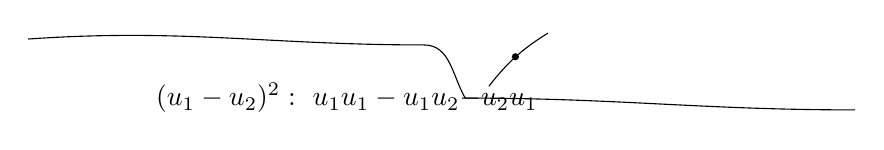
\begin{tikzpicture}[x=.75cm,y=.75cm]
\node[anchor=west] at (2,.1) {$(u_1-u_2)^2:\ u_1u_1-u_1u_2\unsure{-u_2u_1}$};
\draw (0,1.1) to[out=4,in=180] (6.7,1) to[out=0,in=120] (7.4,.1) to[out=0,in=180] (14,-.1);
\draw (7.8,.3) to[bend left=10] (8.8,1.2);\fill (8.25,.8) circle (.06);
\end{tikzpicture}}
\[\sum 1_{x_0,x_1}\qquad u_1\]
\diagram{\begin{tikzcd}[ampersand replacement=\&]
A_{c'}\times A_c\arrow[r]\&A_{c'c}
\end{tikzcd}}
si \uuline{$c'$ et $c$ \unsure{composables}} (\unsure{en cet ordre})
\figure{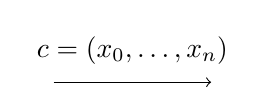
\begin{tikzpicture}
\node at (2,.4) {$c=(x_0,\ldots,x_n)$};\draw[->] (1,0)--(3,0);
\end{tikzpicture}}
\[c'=(x_n,\unsure{\ldots},x_m)\]
\[\unsure{u}\mathord{-}\]
\diagram{\begin{tikzcd}[ampersand replacement=\&]
A_{c'}\arrow[r,dash]\&A_{c'c}\\
A_c\arrow[r,dash]\&A_{c'c}
\end{tikzcd}}
\uline{Sinon on prend 0}

\deleted{\unsure{Évidemment}}
\diagram{\begin{tikzcd}[ampersand replacement=\&]
A_{c''}\times A_{c'}\times A_c\arrow[r]\arrow[d]\&A_{c''c'}\times A_c\arrow[d]\\
A_{c''}\unsure{\times}A_{c'c}\arrow[r]\&A_{c''c'c}
\end{tikzcd}}
\[\deleted{\unsure{*}}\]
\diagram{\begin{tikzcd}[ampersand replacement=\&,row sep=large]
f,g,h\arrow[r]\&\bigl(\underbrace{i_{c'',c''c'}(f)i_{c',c''c'}(g)},\ h\bigr)\arrow[d]\\
\&\underbrace{i_{\unsure{c''c'},c''c'c}(\underline{\hspace{1cm}})}_{i_{c'',c''c'c}(f)i_{c',c''c'c}(g)}i_{\unsure{c},c''c'c}(h)
\end{tikzcd}}
\[i_{c'',c''c'c}(f)\ i_{c',c''c'c}(g)\ i_{c,c''c'c}(h)\]
\figure{\begin{tikzpicture}
\draw[->,thick] (0,0)--(1.2,0);\draw (0,-.1)--(0,.1);\node at (.6,.4) {$c$};
\draw[->,very thick] (1.6,0)--(2.9,0);\draw (1.6,-.1)--(1.6,.1);\node at (2.2,.4) {$c'$};
\draw (3.5,0)--(4.7,0);\draw[very thick] (4.7,-.1)--(4.7,.1);\node at (4.1,.4) {$c''$};
\node at (6,0) {$A_c$};
\end{tikzpicture}}
% archive sheet number: 62
